\documentclass{report}

\usepackage[utf8]{inputenc}
\usepackage[T1]{fontenc}
\usepackage{hyperref}
\usepackage{geometry}
\usepackage{graphicx}
\usepackage[T1]{fontenc}
\usepackage{ltablex}
\geometry{hmargin=2.5cm,vmargin=1.5cm}

\begin{document}

\title{MicronetToNMEA}

\chapter {Introduction}

\section{What is MicronetToNMEA}

MicronetToNMEA is a Teensy/Arduino based project aimed at building a cheap NMEA/Micronet bridge. The initial purpose of this project was to understand Micronet wireless protocol and to be able to record wind and speed data on a PC. The understanding of the protocol went so well that MicronetToNMEA is now doing a lot more. It can:

\begin{itemize}
\item Send or receive a NMEA stream to or from your PC/Tablet with data on depth, water speed, wind, magnetic heading, GNSS positioning, speed, time, etc.
\item Send Heading data from the LSM303 navigation compass to your Micronet's displays (HDG).
\item Send GNSS data to your Micronet displays (LAT, LON, TIME, DATE, COG, SOG) and to your PC/Tablet.
\item Send navigation data from your PC/Tablet (OpenCPN, qtVlm, avnav, etc.) to your Micronet displays (BTW, DTW, XTE, ETA).
\end{itemize}

\section{What is NOT MicronetToNMEA}

MicronetToNMEA is not waterproof and more generally not reliable. All electronics used in this project are made for hobbyist and are all but robust. In the brutal, wet and salty environment of a boat, it will likely fail quickly. So be careful that MicronetToNMEA should not be used as primary navigation tool. Also note that Micronet wireless protocol has been reverse engineered and that many of its aspects are not yet properly understood. Worse, some understandings we think to be correct might be false in some circumstances. If you need state of the art and reliable navigation devices, just go to your nearest Raymarine/TackTick reseller.

\section{Contributors}

\begin{itemize}
\item Ronan Demoment : Main author
\item Dietmar Warning : LSM303 drivers \& Bugfixes
\item \href{https://github.com/j-lang}{j-lang} : UBLOX M8N initialization code
\item Contributors of YBW forum's Micronet thread : \href{https://forums.ybw.com/index.php?threads/raymarines-Micronet.539500/}{Micronet Thread}
\end{itemize}

\chapter{Needed hardware and software}

\section{Required hardware}

To work properly, MicronetToNMEA needs at least a Teensy 3.5, 3.6, 4.0 or 4.1 board and a CC1101 based breakout board.

\subsection{Teensy micro-controller}
Teensy board has been chosen as the core micro-controller of the MicronetToNMEA system. This choice has been led by one main reason : the author had one available when he started investigating Micronet protocol. That's indeed a good reason but with time, this board has also proven to be pretty well adapted :

\begin{itemize}
	\item It is small
	\item Teensy software stack is rich and stable
	\item It has a lot of highly configurable peripherals
	\item Teensy 3.5 GPIOs are 5V tolerant
	\item Teensy 3.5, 3.6 and 4.1 have a MicroSD slot for potential recording features
\end{itemize}

In theory, you can port MicronetToNMEA SW to any 32bit Arduino compatible board. Practically, this might be a different story. Several people got into troubles trying to use ESP32 boards. While this is technically feasible, Arduino's library implementation between Teensy \& Esp32 board can be slightly different in some sensitive areas like interrupt handling. This makes porting complex on a software which needs 100us precise interrupt triggers.

Practically, Teensy 4.0 is advised since the author currently use this board. It will help bug investigation if we all have the same hardware.

Teensy boards can be ordered here : \url{https://www.pjrc.com/teensy/}

\subsection{CC1101 board}

CC1101 is mandatory to MicronetToNMEA. It is the IC which enables RF communication with Micronet/TackTick devices. CC1101 breakout boards are very cheap but the quality of design and components is often less than average. So do not expect to have the same distance performance than original TackTick devices. Be careful when ordering this board since it is designed for a specific range of frequencies (filter and antenna), even if the board is announced to support 434 \& 868MHz (the IC can, but the antenna filter can not). MicronetToNMEA needs a board designed for 868/915MHz usage. Ordering the wrong board would dramatically reduce operating distance between MicronetToNMEA and TackTick devices. Here is an example of a suitable board: \href{https://www.amazon.fr/laqiya-cc1101-868-MHz-Transmission-Antenne-Transceiver/dp/B075PFQ57G}{868MHz CC1101 module}

These low-cost boards are often delivered without any documentation, especially pin-out description. In that case CC1101 data-sheet might help : \href{https://www.ti.com/lit/ds/symlink/cc1101.pdf}{CC1101 datasheet}

\section{Optional hardware}

You can add optional HW to MicronetToNMEA to enhance its capabilities.

\subsection{NMEA0183 GNSS}

If you want to connect a GNSS/GPS to MicronetToNMEA, there is only one important point: it must output localization data on a RS232 link using NMEA0183 format. An example of cheap GNSS which fits the need is the UBLOX NEO-M8N. The NEO-M8N can directly output NMEA stream to its serial output. Avoid too cheap offers from unknown HW sources, this might be counterfeit hardware.

\subsection{NMEA0183 AIS}

If you already have an AIS with a NMEA0183 output on your boat you can use it as a GNSS source. MicronetToNMEA also have the capability to forward AIS data to the PC/Tablet. Be careful that AIS outputs are not 3.3V and that you will likely need a level shifter or a RS422/485 transceiver to protect Teensy boards.

\subsection{LSM303DLH or LSM303DLHC navigation compass breakout board}

Connected to Teensy I2C bus, this IC will allow getting magnetic heading. MicronetToNMEA automatically detects the presence and type of LSM303DLH/DLHC on its I2C bus.

\subsection{Wireless serial devices for NMEA link (BT or WiFi)}

You can connect HC-06 bluetooth transceiver to MicronetToNMEA serial NMEA port to easily get a wireless connection to a PC/Tablet. Connecting an ESP8266 based Serial to WiFi board (Wemos, nodeCPU etc.) allow you to establish an WiFi access point and a client connection to navigation software like OpenCPN.

Note that MicronetToNMEA does not configure both boards, it is up to you to configure before connecting it.

\section{Required software}

\subsection{Arduino IDE (required)}
Arduino IDE provides gcc-arm compiler and all libraries necessary for MicronetToNMEA. This is the first software you must install.

\subsection{Teensyduino (required)}

Teensyduino is an extension to Arduino IDE which add full support to all Teensy’s board. It must be installed on top of Arduino IDE to enable compilation for Teensy targets.

\section{Optional software}

\subsection{Visual Studio Code and PlatformIO (optional)}

If you plan to do more than just compile MicronetToNMEA’s code, you probably need a more serious IDE. \href{https://code.visualstudio.com/}{Visual Studio Code} is a open source IDE made by Microsoft with plenty of features which will highly improve your productivity. Coupled to \href{https://platformio.org/}{PlatformIO} plugin it can handle project for Teensy boards. MicronetToNMEA includes configuration files for PlatformIO which will help you to quickly setup your environment.

Note that you don't need Arduino IDE or Teensyduino if you use Visual Studio Code and PlatformIO.

\chapter{Compilation}

\section{With Arduino IDE}

Here are the steps to compile MicronetToNMEA with Arduino IDE:

\begin{itemize}
\item Get the source code from MicronetToNMEA repository (\url{https://github.com/Rodemfr/MicronetToNMEA})
\item Double-click on src/src.ino. This should open Arduino IDE.
\item In Arduino IDE, select the appropriate Teensy board with menu “Tools->Board->Teensyduino->Teensy4.0”
\item Go to menu “Tools->Manage Libraries...” and install TeensyTimerTool library
\item Click on “Verify” button in the button bar, this should compile the project without error.
\item Connect your Teensy board onto USB port of your PC and Click “Upload” button to upload MicronetToNMEA binary into Teensy flash memory
\end{itemize}

\section{With Visual Studio Code and PlatformIO}

Here are the steps to compile MicronetToNMEA with Visual Studio Code :

\begin{itemize}
\item Install Visual Studio Code from Microsoft website : \url{https://code.visualstudio.com}
\item Start Visual Studio Code and install PlatformIO extension. Note that you might have to install \emph{python3-distutils} package under Linux for the installation to be successful.
\item Open MicronetToNMEA base folder with menu \emph{"File->Open Folder"}. The base folder is the one with \emph{platformio.ini} file.
\item At the first opening, PlatformIO plugin will download and install Teensy toolchain. This can take a while since there is more than 1Gb of data to download from network.
\item Once PlatformIO is ready, you can compile MicronetToNMEA by pressing \emph{SHIFT-CTRL-B}.
\item To upload the compiled binary to the Teensy, press \emph{SHIFT-CTRL-U}.
\end{itemize}

Your project should compile now.

\section{Compile time configuration}
\label{compile-time-configuration}

By default, MicronetToNMEA is configured for a specific HW layout. This means that it is configured to be connected through specific SPI, I2C or GPIO pins to various boards. This configuration can be changed to some extent to adapt your own needs. The file bearing this configuration is “BoardConfig.h”. Note that no coherency check is made in the software, it is your responsibility to provide a reachable configuration (i.e. not to connect SPI wires to non SPI capable pins). Table {\ref{table:configswitches}} lists all available switches and their meaning.

	\begin{tabularx}{\linewidth}{@{}lX@{}}
		\hline
		\textbf{Compile Switch} & \textbf{Description}\\
		\hline
		FREQUENCY\_SYSTEM & Defines which frequency range is used by your Micronet network (0=868MHz, 1=915MHz)\\
		\hline
		NAVCOMPASS\_I2C & Sets the I2C bus to which the navigation compass (i.e. LSM303DLH(C)) is connected. Defined as per “Wiring” library definition (Wire0, Wire1, etc.)\\
		\hline
		CS0\_PIN & Defines SPI Chip Select line connected to RF IC\\
		\hline
		MOSI\_PIN & Defines MOSI pin of SPI bus connected to RF IC\\
		\hline
		MISO\_PIN & Defines MISO pin of SPI bus connected to RF IC\\
		\hline
		SCK\_PIN & Defines SCK pin of SPI bus connected to RF IC\\
		\hline
		GDO0\_PIN & Defines GDO0 pin of SPI bus connected to RF IC\\
		\hline
		LED\_PIN & Defines the pin driving the LED, which is used for error signaling\\
		\hline
		GNSS\_UBLOXM8N & Enable automatic configuration of UBLOX M8N GPS (0=disabled, 1=enabled)\\
		\hline
		GNSS\_SERIAL & Defines on which serial port is connected the NMEA GNSS (Serial, Serial1, Serial2, etc.)\\
		\hline
		GNSS\_BAUDRATE & Defines GNSS UART default baud-rate\\
		\hline
		GNSS\_RX\_PIN & Defines serial RX pin connected to NMEA GNSS TX pin\\
		\hline
		GNSS\_TX\_PIN & Defines serial TX pin connected to NMEA GNSS RX pin\\
		\hline
		USB\_NMEA & Defines which serial port is connected to the USB NMEA connection\\
		\hline
		USB\_BAUDRATE & Defines baud rate of USB serial converter\\
		\hline
		WIRED\_NMEA & Defines which serial port is connected to the wired NMEA connection\\
		\hline
		WIRED\_BAUDRATE & Defines baud rate of the wired NMEA connection\\
		\hline
		WIRED\_RX\_PIN & Defines serial RX pin used for wired NMEA\\
		\hline
		WIRED\_TX\_PIN & Defines serial TX pin used for wired NMEA\\
		\hline
		CONSOLE & Defines on which serial port is displayed the console (can be USB\_NMEA or WIRED\_NMEA). Can be on the same serial link than NMEA\_EXT\\
		\hline
		NMEA\_EXT & Defines to which serial port is connected the external NMEA stream. (can be USB\_NMEA or WIRED\_NMEA). Can be on the same serial link than CONSOLE and NMEA\_IN.\\
		\hline
		NAV\_SOURCE\_LINK & Defines where navigation data is coming from (related to RMB sentences). See Section {\ref{supportednmeasentences}} for more details on possible values.\\
		\hline
		GNSS\_SOURCE\_LINK & Defines where positioning data is coming from (related to RMC, GGA, VTG sentences). See Section {\ref{supportednmeasentences}} for more details on possible values.\\
		\hline
		WIND\_SOURCE\_LINK & Defines where wind data is coming from (related to MWV sentence). See Section {\ref{supportednmeasentences}} for more details on possible values.\\
		\hline
		DEPTH\_SOURCE\_LINK & Defines where depth data is coming from (related to DPT sentence). See Section {\ref{supportednmeasentences}} for more details on possible values.\\
		\hline
		SPEED\_SOURCE\_LINK & Defines where speed data is coming from (related to SPD, LOG sentences). See Section {\ref{supportednmeasentences}} for more details on possible values.\\
		\hline
		VOLTAGE\_SOURCE\_LINK & Defines where voltage data is coming from (related to XDR sentence). See Section {\ref{supportednmeasentences}} for more details on possible values.\\
		\hline
		SEATEMP\_SOURCE\_LINK & Defines where temperature data is coming from (related to STP sentence). See Section {\ref{supportednmeasentences}} for more details on possible values.\\
		\hline
		COMPASS\_SOURCE\_LINK & Defines where heading data data is coming from (related to HDG sentence). See Section {\ref{supportednmeasentences}} for more details on possible values.\\
		\hline
		SOG\_COG\_FILTERING\_ENABLE & If set to 1, MicronetToNMEA will filter SOG and COG values before sending them to Micronet displays or to NMEA\_EXT link. \\
		\hline
		SOG\_COG\_FILTERING\_DEPTH & Sets the strength of the SOG/COG filtering, if enabled. Minimum value is 1 (no filtering), maximum reasonable value is 20 (average on 20 samples). Default is set to 7.\\
		\hline
		EMULATE\_SPD\_WITH\_SOG & If set to 1, MicronetToNMEA will copy SOG value received from GNSS to SPD on the Micronet network. Not to be used if you have water speed measurements coming from T121 or NMEA. \\
		\hline
\end{tabularx}
\begin{table}[h]
	\caption{Configuration switches in BoardConfig.h}
\label{table:configswitches}
\end{table}

\chapter{Installation}

Teensy board must be connected to other boards with the same scheme than you have defined in “BoardConfig.h”. No check is made by MicronetToNMEA software to verify that your configuration is matching your actual connections. You must carefully verify that you properly connected the various devices since wrong connections can possibly damage your hardware, especially with respect to power supply connections which are mixing 3.3 \& 5V levels.

\section{Power supply}

The first and most important connection to build is the power supply. You have two options there, you can either :

\begin{itemize}
	\item Power the system via USB
	\item Power the system using external DC power source
\end{itemize}

\subsection{Power via USB}

This is the most straightforward way to power the system: just plug an USB cable in the Teensy connector and it will be powered by the connected PC. Teensy board is equipped with a voltage regulator which provides 3.3V. This 3.3V voltage can be used to power other boards of the system.
Be careful that USB 2.0 limits 5V output current to 500mA, but you should be even more careful since Teensy's regulator recommends not to exceed 250mA for 3.3V. So you must take care that your system does not exceed these limits.
As an example, table \ref{table:boardconsumption} shows maximum current values for various boards.

\begin{table}[h]
	\begin{tabular}{|l|c|c|l|}
		\hline
		Board & Supply voltage & Max current & Comment \\
		\hline
		Teensy 3.5 & 5V & 50mA & CPU running at 120MHz\\
		Teensy 3.6 & 5V & 80mA & Input not 5V tolerant\\
		Teensy 4.1 & 5V & 100mA & Input not 5V tolerant\\
		CC1101 & 3.3V & 40mA & RF at 868MHz\\
		NEO M8N GNSS & 5V & 45mA & IOs are 3.3V\\
		LSM303DLH(C) & 3.3V & 10mA & Unspecified in datasheet, value assumed\\
		HC06 Bluetooth transceiver & 3.3V & 40mA & Peak during pairing\\
		Serial WiFi (ESP8266) & 5V & 150mA & 80mA average, upto 400mA peak\\
		\hline
	\end{tabular}
	\caption{Current consumption of typical boards}
	\label{table:boardconsumption}
\end{table}
USB powering is especially useful when you plan to output NMEA through USB-serial. In this case, the connected PC/Tablet will provide power to the system and when MicronetToNMEA is not needed anymore, just unplug the USB cable to power-off the system.

\subsection{Power with an external DC source}
While USB powering is easy to setup, it is not a common source of power in a boat. It is more usual to get two wires with an unstable battery voltage between 11V and 15V. In that case, you will need a voltage regulator or a DC-DC converter which will be used to produce a stable 5V for the system. This 5V source can then be connected to the Vin pin of Teensy. The on-board regulator will then produce 3.3V from this input.
\linebreak
When Vin pin is connected to an external source of power, you must not connect an USB cable to avoid short circuit between Vin and Vusb which are connected together on Teensy by default. The Vin pin can handle voltages from 3.6 to 6V but it is strongly recommended to use 5V here. This way, if you accidentally connect a USB cable while powering Vin, there will be no heavy short circuit.

\begin{figure}
\centering

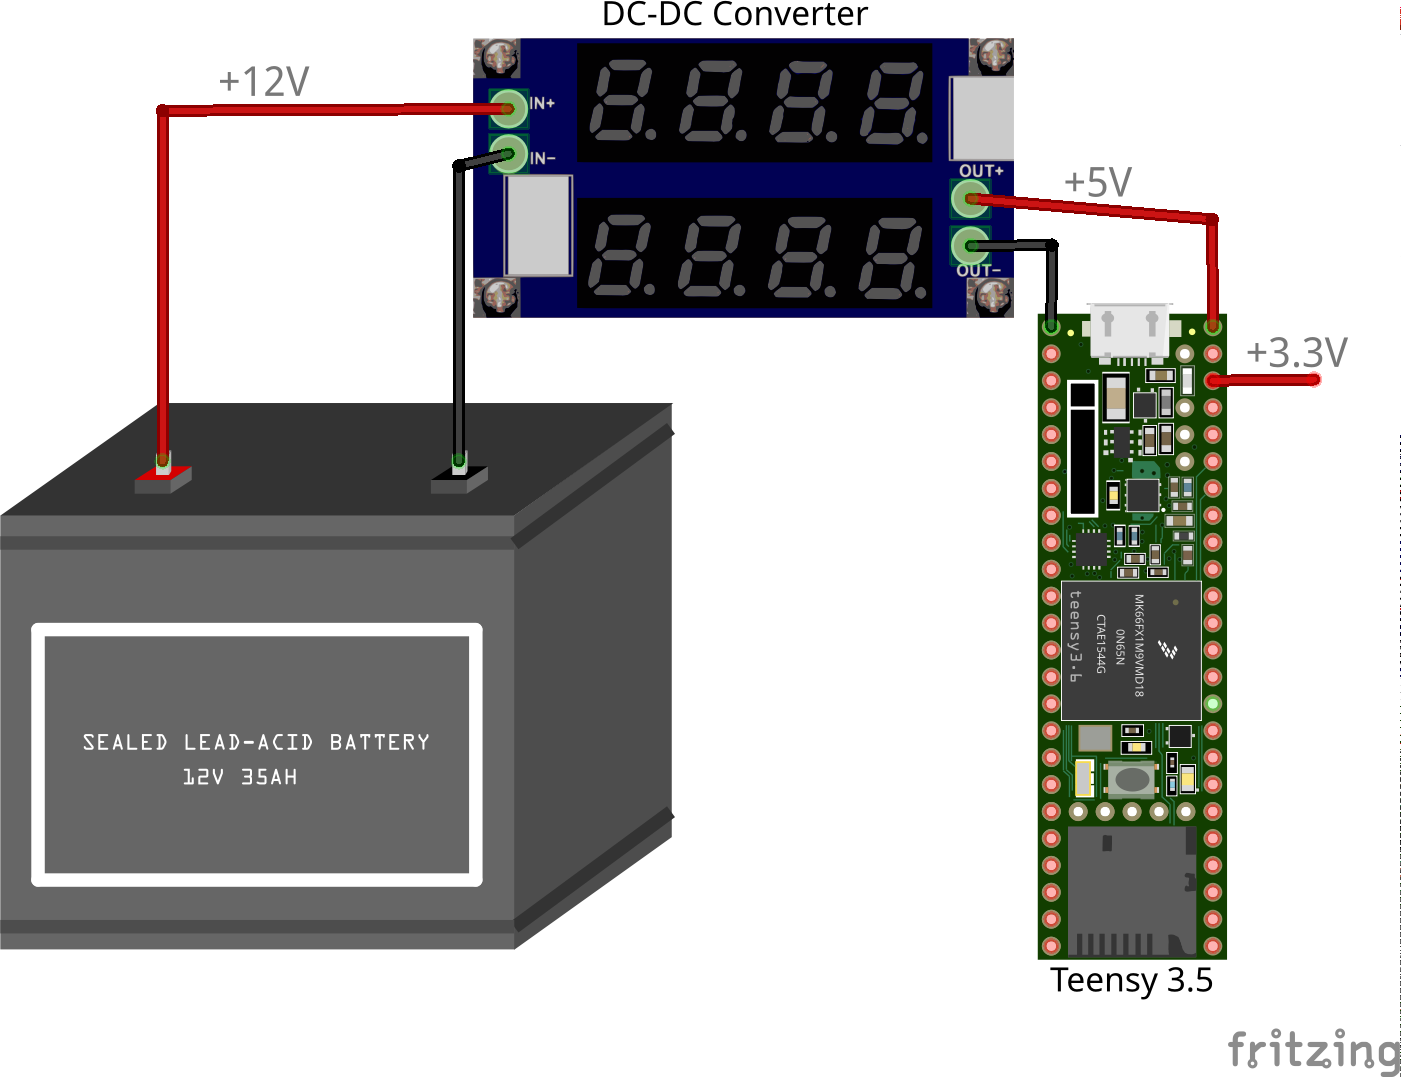
\includegraphics[width=100mm]{MicronetToNMEA_DC_Power.png}
	\caption{Powering Teensy with a DC-DC converter}
\label{figure:dcpower}
\end{figure}

\section{Connecting CC1101}

CC1101 uses 3.3V voltage so you can connect Teensy's 3.3V \& GND pins to CC1101's VCC \& GND. MOSI(SI), MISO(SO), CS0 and GD0 must be connected as per your BoardConfig.h definitions. Note that GDO2 isn't used by MicronetToNMEA and doesn't need to be connected to Teensy. Figure \ref{figure:cc1101} shows how to connect CC1101 with the default configuration.

\begin{figure}[h]
	\centering
	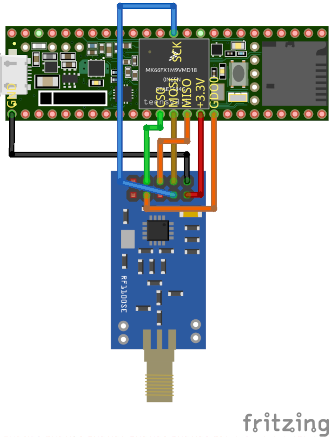
\includegraphics[width=50mm]{MicronetToNMEA_CC1101.png}
	\caption{Connecting Teensy and CC1101}
	\label{figure:cc1101}
\end{figure}

\section{Connecting LSM303}

LSM303DLH(C) uses 3.3V voltage so you can connect Teensy's 3.3V \& GND pins to CC1101's VCC \& GND. In addition SDA \& SCL must be connected as per your BoardConfig.h definitions. Note that DRDY, I1 \& I2 don't need to be connected. Figure \ref{figure:lsm303} shows how to connect LSM303DLH(C) with the default configuration.

\begin{figure}[h]
	\centering
	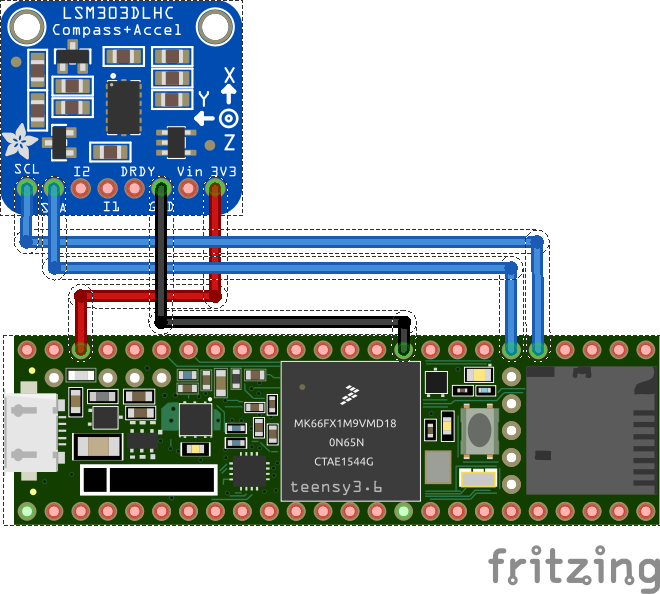
\includegraphics[width=50mm]{MicronetToNMEA_LSM303.png}
	\caption{Connecting Teensy to LSM303}
	\label{figure:lsm303}
\end{figure}

\section{Connecting GNSS}

Unlike CC1101 or LSM303DLH(C), GNSS/GPS boards are often requiring 5V VCC as power voltage. So you have to connect it directly to DC-DC Converter's output. You should check however that your GNSS board is not 3.3V powered, in which case you should use one of Teensy 3.3V pin.
TX and RX pins must then be connected respectively on RX and TX of Teensy's UART. The recommended UBLOX M8N module has an internal regulator to 3.3V on board, so you can connect GNSS directly even if it is using 5V supply voltage. This situation may be different for other GNSS modules. 

Figure \ref{figure:gnss} shows how to connect GNSS for the default configuration.

\begin{figure}[h]
	\centering
	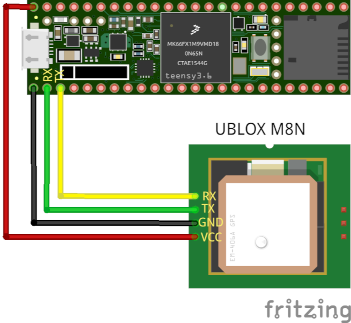
\includegraphics[width=50mm]{MicronetToNMEA_GNSS.png}
	\caption{Connecting Teensy and GNSS}
	\label{figure:gnss}
\end{figure}

MicronetToNMEA can connect to a wide variety of GNSS. You just have to configure the GNSS with the correct parameters before connecting it. GNSS has to output an NMEA compatible stream at the same bit-rate than specified in BoardConfig.h. MicronetToNMEA can automatically configure the GNSS if it is a UBLOX Neo M8N. Just enable GNSS\_UBLOXM8N option in BoardConfig.h.

GNSS should output the following sentences :
\begin{itemize}
	\item GGA : Position
	\item RMC : Time
	\item VTG : Track and speed
\end{itemize}

\section{Connecting wireless serial modules}

When MicronetToNMEA is configured to send its console and/or NMEA
output to a standard wired UART (i.e not USB), you can consider connecting
a HC-06 Bluetooth transceiver or an Serial WiFi board to easily get
wireless connectivity to your PC/Tablet. Both boards are powered with
5V but can handle 3.3V signals. Only VCC, GND, RXD \& TXD need to
be connected. Figure \ref{figure:hc06} shows how to connect e.g.
HC-06 with the default configuration.

\begin{figure}[h]
	\centering
	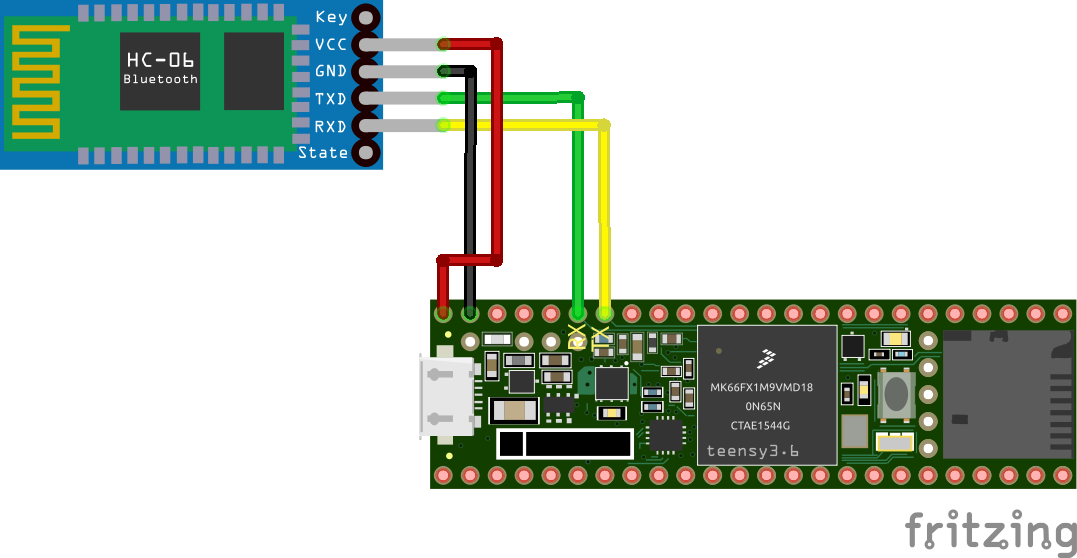
\includegraphics[width=85mm]{MicronetToNMEA_HC06.png}
	\caption{Connecting Teensy and HC-06}
	\label{figure:hc06}
\end{figure}

As for the GNSS, MicronetToNMEA does not configure HC-06 itself. It is your responsibility to configure HC-06 properly (i.e. with parameters matching BoardConfig.h) prior to connecting it to Teensy.

\section{Recommendations}

\subsection{RF performance}
Micronet devices cannot legally exceed a handful of milliwatts of transmit power. As a consequence the operational range will hardly exceed 15-20m. It is important not to put metal objects or panels between your various devices. This would dramatically reduce of the operational range of MicronetToNMEA.
You should also be careful if you are racing and using carbon sails. If the sails are between your wind vane and MicronetToNMEA, you will likely not receive wind data. Carbon disturbs RF transmissions.
It is generally considered not to be a good idea to use wireless electronics in a carbon boat or with carbon sails. Fibreglass attenuates only a little the signal, so it is safe to attach your device inside a GRP hull.

The quality of CC1101's antenna is critical to maximize RF performance and operational range. Antennas provided with low cost breakout boards are often designed to be small at the cost of RF performance. An easy way to get a good quality antenna is to use a simple electrical wire with the adequate length (quarter wavelength: 86.5mm for 869MHz or 82mm for 915MHz). With such an antenna you can reach a very good operating range. Wire antenna also have the interesting feature of beeing flexible so that you can orient them to maximize wind reception (use \emph{"Test RF quality"} menu for that).

\subsection{Magnetic compass disturbances}
\label{compass-recommendations}
If your are using LSM303 to get magnetic heading, it is very important to put your MicronetToNMEA assembly far from other electrical devices, especially those carrying a bit of power. This can highly disturb magnetic compass. As an example, a running 24" TV monitor can deviate the compass by 20° at 50cm and still a few degrees at 1m.
Also, metal must be avoided : it deviates magnetic field. The bigger the piece of metal is the farthest you should put your device. In a boat you should avoid the keel, batteries and the inboard engine. At a smaller scale, you should keep LSM303 board away from DC-DC converter if you can.

\subsection{Magnetic compass calibration}
An electronic compass must be properly calibrated to produce good values. The theory tells us that a perfect calibration would need to have your device attached in its final position and to spin your boat around the 3 axis. This is generally not something we want to do. To achieve a good calibration with less complex operations, the best is to calibrate MicronetToNMEA outside your boat, far from any metal or electronic device. You should also keep it as far as possible of its power supply. Once calibrated, get it back to your boat and fix it in a proper place, following the above recommendations. This should give good results.

\subsection{CPU frequency and power consumption}
The latest Teensy boards have powerful CPUs running up to 600MHz. This power has a cost : power consumption. MicronetToNMEA doesn't need so much power so it is advised to reduce the CPU speed to 24MHz. It will significantly reduce power consumption.
On a system with a Teensy 4.0@24MHz, a NEO M8M GNSS, a HC-06 Bluetooth transceiver, a CC1101, a LSM303DLH and a oversized DC-DC converter, the complete power consumption at 12V connector is averaging around 850mW (700-1000mW).

\chapter{Usage}

\section{Configuring MicronetToNMEA}

\subsection{Connecting to the console}

To be able to configure MicronetToNMEA, you must have access to the configuration menu displayed on the serial console. By default, this console is connected to the USB serial port of Teensy. So you just have to find a terminal software to connect to it. A good open source terminal is \href{http://www.teraterm.org/}{Tera Term}. Note that when using Teensy USB connection, you can use any baud-rate on PC side, this as no real effect.

At the first power-up, before having configured MicronetToNMEA, console should go directly to the configuration menu. If this is not the case, it means that a configuration as already been written in EEPROM and that MicronetToNMEA has automatically switched to "NMEA conversion mode". In this case, you just have to press \emph{<ESC>} key to come back to the configuration menu.

The menu should look like this :

\begin{verbatim}
*** MicronetToNMEA ***

0 - Print this menu
1 - General info on MicronetToNMEA
2 - Scan Micronet networks
3 - Attach converter to a network
4 - Start NMEA conversion
5 - Scan surrounding Micronet traffic
6 - Calibrate RF XTAL
7 - Calibrate compass
8 - Test RF quality
\end{verbatim}

\subsection{Attaching your Micronet network to MicronetToNMEA}

We need to identify your Micronet network for MicronetToNMEA to be able to recognize it and to ignore other networks that may be in you vicinity. You will typically find several networks when in a marina with many sailing boats.
To identify your network, you have to power-up your Micronet display and to ensure that your master device, the one you used to power-up the network, is close to MicronetToNMEA, let say, 2 or 3 meters maximum. Once done, enter \emph{"2 - Scan Micronet networks"} menu by pressing 2 in the console. This will start a five second scanning sequence which listens to every network in the area. At the end of this sequence, every network found will be listed in the console. If there are several networks, they are listed in decreasing order of power.

\begin{verbatim}
Network - 83038F54 (very strong)
Network - 810278A6 (low)
\end{verbatim}

Yours is very likely at the top of the list with mention "very strong". This is the signal strength. For each network you get a hexadecimal number which is the so called "Network ID". Write it on a piece of paper (\emph{83038F54} in our example).
Now enter menu \emph{"3 - Attach converter to a network"} by pressing 3, and type your network ID when requested. This will attach MicronetToNMEA to your Micronet network.
Once done, MicronetToNMEA will save this value to EEPROM and will remember it. You don't need to do this operation at each start-up. Now that MicronetToNMEA is attached, it will automatically go to NMEA conversion mode at the next power-up.

\subsection{Calibrating CC1101 RF XTAL}

CC1101 board uses a crystal to generate its frequencies. Crystal frequency is more or less precise and needs to be calibrated for CC1101 to generate exactly the expected frequency. Each crystal needs to be calibrated independently. This calibration is very important because it directly influences the range performance of the RF system (i.e. the maximum distance at which MicronetToNMEA can detect other devices). When you buy a TackTick device, this calibration has already been done at factory. But when you build a MicronetToNMEA system, you need to do it yourself.

Menu \emph{"6 - Calibrate RF XTAL"} does this calibration. Enter it by pressing key 6. A text will explain the procedure : power-up your Micronet network and place the master device (the one you used to power-up the network) very close to MicronetToNMEA (less than one meter). Now press any key and let the calibration proceed. During 2 minutes, you will see dots and stars appear on the console looking like this :

\begin{verbatim}
...................*.**********************.**.....................................
\end{verbatim}

Each character represents a tested frequency where MicronetToNMEA verifies if it receives data from the Master device. A dot means that nothing was received, a star means that a message was received. The center of the starred area is the best reception frequency and MicronetToNMEA will use this one to get the best RF performance. Your crystal is calibrated.
At the end of the procedure, you will be asked if you want to save the new calibration value to EEPROM. Just answer yes and your calibration will be done once for all.

\subsection{Calibrating navigation compass}

Navigation compass needs to be calibrated on its 3 axis to produce correct heading measurements. An uncalibrated compass will give totally wrong values and not just by a few degrees.

The base principle of calibration consists in determining the minimum and maximum values of earth's magnetic field onto each of the three axis of the sensor. This way, heading calculation will be able to remove any bias on the 3 axis. This bias is produced by the LSM303 itself, but also by surrounding electronics (Teensy, GNSS, etc.).

Before starting calibration, you must first prepare your environment as explained in \ref{compass-recommendations}. Once ready, you can enter menu \emph{"7 - Calibrate compass"}.

This menu will produce a permanent output of calibration values looking like this :

\begin{verbatim}
(0.2 -0.35 -0.17)
[0.20 0.98] [0.12 1.0] [-0.25 0.99]
\end{verbatim}

The first line gives the current magnetic field on each of the three axis : X, Y and Z.
The second line gives the two calibration parameters for each axis : center value ((max + min) / 2) and axis amplitude (max - min).

Your objective for a successful calibration is to maximize/minimize readings on each axis. To do this, you must first choose one axis and then rotate your MicronetToNMEA device until this axis is aligned with earth's magnetic field vector. You should see the corresponding reading on the first line maximum (or minimum).
You must repeat this operation a second time for the same axis but for opposite values (i.e. you must minimize the reading). Each time you reach the maximized/minimized value, you don't need to do anything, MicronetToNMEA will memorize the min/max values for each axis.

Note that the magnetic field vector is pointing more or less to the north, but not horizontally, it is pointing somewhat down to earth in north hemisphere and up to the sky in south hemisphere.

You must reproduce this operation for all 3 axis to complete calibration.
A successful calibration should lead to very close amplitude values for all 3 axis, on the second line. Center values can however be very different.

Once achieved, just press \emph{<ESC>} and tell MicronetToNMEA to save the value in EEPROM. Your compass is calibrated.

\subsection{Testing RF performance}

Menu \emph{"8 - Test RF quality"} will help you to evaluate the quality of the connection with each Micronet devices individually. This will be critical to fix your MicronetToNMEA assembly at the right place in your boat. When entering this menu, you will see the list of devices of your network with a indicator of the connection quality :

\begin{verbatim}
81071e60 LNK=7.6 NET=9 Dual Display [M]
01071e77 LNK=7.2 NET=9 Hull
81037082 LNK=6.2 NET=7 Dual Display
83037737 LNK=6.2 NET=6 Wind Display
830ab252 LNK=6.2 NET=9 Wind Display
\end{verbatim}

\emph{LNK} indicates the strength of the signal of the device as received by MicronetToNMEA.

\emph{NET} indicates the strength of the signal of the Master as received by the device.

A value of 9 is considered excellent while a value below 3 is low. \emph{LNK} can be used to find the best place for MicronetToNMEA, while \emph{NET} is useful to check if every device is properly receiving master's messages. The list is refreshed every second. The problematic device is generally the wind transducer which is shadowed by the mast. Placing MicronetToNMEA and your master display outside this shadow will ensure a good wind reception.

\subsection{Starting NMEA conversion}

Menu \emph{"4 - Start NMEA conversion"} actually start Micronet/NMEA conversion as suggested by the name. Once you enter in this mode MicronetToNMEA will output NMEA sentences to the NMEA\_EXT link. By default, NMEA\_EXT is routed to the same serial link than the console (USB serial). It means that you will immediately see NMEA sentences beeing written onto console. Additionnaly, MicronetToNMEA also decodes any incoming NMEA sentence from NMEA\_EXT serial and transmits it to your Micronet network.
You need to be in this mode to see decoded GNSS or NMEA data displayed onto your Micronet displays. You also need to be in this mode for the configuration parameters modified onto your Micronet displays to be memorized by MicronetToNMEA (e.g. speed factor, sounder offset, etc.).
If attached to a network, MicronetToNMEA will automatically switch to this mode when powered-up. You can leave it by just pressing \emph{<ESC>} in the console.
\\
\\
Here is a summary of all actions realized by MicronetToNMEA in this mode, with the default configuration :
\begin{itemize}
	\item Collect and decode GNSS related NMEA sentences from GNSS\_NMEA link
	\item Collect and decode navigation related NMEA sentences from NMEA\_EXT link
	\item Forward GNSS related NMEA sentences from GNSS\_NMEA link to NMEA\_EXT link
	\item Forward AIS related NMEA sentences from GNSS\_NMEA link to NMEA\_EXT link is an AIS is used to get GNSS data
	\item Collect and decode data from Micronet devices
	\item Send all data collected from NMEA links to Micronet network
	\item Send all data collected from Micronet devices to NMEA\_EXT link
	\item Calculate heading from LSM303DLH(C)
	\item Send heading data to Micronet network and NMEA\_EXT link
\end{itemize}

It is important to note that the configuration can change this sequence and the way MicronetToNMEA decodes/forwards data. See chapter {\ref{supportednmeasentences}} for more details.

\subsection{NMEA sentences and data flow}\label{supportednmeasentences}

MicronetToNMEA handles a number of data fields coming either from Micronet network, either from NMEA links.
NMEA sentences can be handled in various ways depending on your installation. MicronetToNMEA offers the possibility to configure how Micronet data and NMEA sentences are processed. NMEA sentences can be configured to be decoded/encoded from the following links :
\begin{itemize}
	\item LINK\_MICRONET : This link accesses data of the Micronet newtork through CC1101 IC. If a sentence is configured to be received from this link, it means that it will be decoded every second from Micronet data and sent to NMEA\_EXT link.
	\item LINK\_NMEA\_GNSS : This is the NMEA link with the optional GNSS or AIS. It is a receiving only link. If a sentence is configured to be received from this link, it means that it will be decoded and sent to Micronet network. It will also be forwarded to NMEA\_EXT.
	\item LINK\_NMEA\_EXT : This is the NMEA link with the "external" device. The external device can be a PC with a navigation software, a WiFi or Bluetooth bridge, etc. Practically it uses NMEA\_IN and NMEA\_OUT serial links defined in BoardConfig.h. If a sentence is configured to be received from this link, it means that it will be decoded and sent to Micronet network.
	\item LINK\_COMPASS : This is the I2C link with LSM303DLH(C) optional IC. If a sentence is configured to be received from this link, it means that it will be sent to Micronet network, then encoded to NMEA\_EXT. 
\end{itemize}

The following table summarizes all supported NMEA sentences, the corresponding Micronet data and the possible source links:

\begin{table}[h]
	\small
	\begin{tabular}{|l|c|c|p{5cm}|}
		\hline
		\textbf{Sentence} & \textbf{Action}  & \textbf{Corresponding Micronet data} & \textbf{Possible sources} \\
		\hline
		RMB & Decoded & XTE DTW BTW VMGWP & LINK\_NMEA\_EXT \\
		\hline
		RMC & Decoded/Forwarded & TIME DATE & LINK\_NMEA\_GNSS LINK\_NMEA\_EXT \\
		\hline
		GGA & Decoded/Forwarded & LAT LON & LINK\_NMEA\_GNSS LINK\_NMEA\_EXT \\
		\hline
		GLL & Decoded/Forwarded & LAT LON & LINK\_NMEA\_GNSS LINK\_NMEA\_EXT \\
		\hline
		VTG & Decoded/Forwarded & COG SOG & LINK\_NMEA\_GNSS LINK\_NMEA\_EXT \\
		\hline
		MWV & Decoded/Encoded & AWA AWS TWA TWS & LINK\_MICRONET LINK\_NMEA\_EXT \\
		\hline
		DPT & Decoded/Encoded & DPT & LINK\_MICRONET LINK\_NMEA\_EXT \\
		\hline
		MTW & Decoded/Encoded & STP & LINK\_MICRONET LINK\_NMEA\_EXT \\
		\hline
		VLW & Decoded/Encoded & LOG TRIP & LINK\_MICRONET LINK\_NMEA\_EXT \\
		\hline
		VHW & Decoded/Encoded & SPD & LINK\_MICRONET LINK\_NMEA\_EXT \\
		\hline
		HDG & Decoded/Encoded & HDG & LINK\_MICRONET LINK\_NMEA\_EXT LINK\_COMPASS \\
		\hline
		XDR & Decoded & VCC & LINK\_MICRONET \\
		\hline
		VDM & Forwarded & None & LINK\_NMEA\_GNSS \\
		\hline
		VDO & Forwarded & None & LINK\_NMEA\_GNSS \\
		\hline
	\end{tabular}
	\caption{Supported NMEA sentences}
	\label{table:nmeasentences}
\end{table}

\end{document}